% Formelsammlung für Elektrotechnik ZHAW

% Dokumenteinstellungen
% ======================================================================

% Dokumentklasse (Schriftgröße 6, DIN A4, Artikel)
\documentclass[6pt,a4paper]{scrartcl}

% Zusätzliche Pakete laden
\usepackage[utf8]{inputenc}        % Zeichenkodierung: UTF-8 (für Umlaute)
\usepackage[german]{babel}        % Deutsche Sprache
\usepackage{multicol}            % Spaltenpaket
\usepackage{amsmath}            % erlaubt mathematische Formeln
\usepackage{amssymb}            % Verschiedene Symbole
\usepackage{esint}                % erweiterte Integralsymbole
\usepackage{booktabs}            % bessere Tabellenlinien
\usepackage{graphicx}            % Zum Bilder einfügen benötigt
\usepackage{color}                % Farbiger Text möglich
\usepackage{pbox}                % Intelligent parbox: \pbox{maximum width}{blabalbalb \\ blabal}
%\usepackage{undertilde}            % Für Welle unterhlab von Matrixbuchstaben benötigt
\usepackage{accents}            % Für eigene Ableitungspunkte benötigt
\usepackage{scrtime}
\usepackage{supertabular}        % Für lange Tabellen mit Umbruch
\usepackage{pdfpages}
\usepackage{trfsigns}            % Laplace und Fourier
\usepackage{array}


% Seitenlayout und Ränder:
\usepackage{geometry}
\geometry{a4paper,landscape, left=6mm,right=6mm, top=-1mm, bottom=3mm,includeheadfoot}
\setlength{\parindent}{0mm}


% Dokumentbeschreibung
\title{Formelsammlung Elektrotechnik ZHAW}
\author{Andreas Sprecher}


% Kopf- und Fußzeile
% ======================================================================
\usepackage{fancyhdr}
\pagestyle{fancy}
\fancyhf{}
   \fancyfoot[C]{\textbf{Elektrotechnik}}
   \renewcommand{\headrulewidth}{0.0pt} %obere Linie ausblenden
   \renewcommand{\footrulewidth}{0.1pt} %obere Linie ausblenden

   \fancyfoot[R]{Stand: \todayV}
   \fancyfoot[L]{Andreas Sprecher}
% ----------------------------------------------------------------------

% Ausgegraut zum Abschreiben:
%\definecolor{grey}{rgb}{0.6,0.6,0.6}
%\color{grey}

% Eigene Befehle und Befehlsüberschreibungen
% ======================================================================

% Schriftart SANS für bessere Lesbarkeit bei kleiner Schrift
\renewcommand{\familydefault}{\sfdefault}
% Array- und Tabellenabstände vergrößern
\renewcommand{\arraystretch}{1.2}

% Befehle sichern
\let\oldvec = \vec
\let\olddot = \dot

% Eigene Befehle
\newcommand{\todayV}{\the\day.\the\month.\the\year}                          %%D.M.YYYY

\newcommand{\iset}[2]{\ensuremath{\bigl\{ \bigl. #1 \, \bigr| \, #2 \bigr\}}}                   % intensional set
\newcommand{\eset}[1]{\ensuremath{\bigl\{#1\bigr\}}}                                            % extensional set
%\newcommand{\enbrace}[1]{\ensuremath{\bigl\(#1\bigr\)}}                                        % extensional set
\newcommand{\enbrace}[1]{\ensuremath{\left(#1\right)}}
\newcommand{\norm}[1]{\ensuremath{\|#1\|}}                                                      % Norm
\newcommand{\mat}[1]{\ensuremath{\begin{bmatrix} #1 \end{bmatrix}}}                             % Matrix
\newcommand{\ma}[1]{\ensuremath{\boldsymbol {#1}}}                                              % Matrixsymbol
\newcommand{\vect}[1]{\ensuremath{\begin{pmatrix} #1 \end{pmatrix}}}                            % Vektor
\newcommand{\mvect}[1]{\ensuremath{\left. \begin{matrix} #1 \end{matrix}  \right]}}             % Matrixvektornotation
\newcommand{\gk}[1]{\ensuremath{\left\lfloor#1\right\rfloor}}                                   % Gaußklammer
\newcommand{\sprod}[2]{\ensuremath{\left\langle #1, #2 \right\rangle }}                         % Skalarprodukt
\newcommand{\abs}[1]{\ensuremath{\left\vert#1\right\vert}}                                      % Betrag
\newcommand{\bdot}{\ensuremath{\boldsymbol \cdot}}                                              % Dicker Punkt für Skalarprodukt
\newcommand{\svdots}{\ensuremath{\olddot :}}                                                    % small vertical dots
\newcommand{\mustbe}{\stackrel{!}{=}}

\newcommand{\inn}{\operatorname{int}}


% Überschreibungen
\renewcommand{\vec}[1]{\ensuremath{\boldsymbol {#1}}}                                           % Vektor fett und unterstrichen
\renewcommand{\emph}[1]{\textbf{#1}}                                                            % Hervorhebungen fett
\renewcommand*{\dot}[1]{\accentset{\mbox{\textrm{\large\bfseries .}} }{#1}}                     % Dicker Ableitungspunkt
\renewcommand*{\ddot}[1]{\accentset{\mbox{\textrm{\large\bfseries .\hspace{-0.25ex}.}}}{#1}}    % Dicker Doppelableitungspunkt

% Abkürzungen
\newcommand{\ul}[1]{\ensuremath{\underline{#1}}}                               % Untersteichen
\newcommand{\ol}[1]{\ensuremath{\overline{#1}}}                                % Überstreichen
\newcommand{\Ra}[0]{\ensuremath{\Rightarrow}}                                  % Rightarrow
\newcommand{\ra}[0]{\ensuremath{\rightarrow}}                                  % Rightarrow
\newcommand{\bs}[1]{\ensuremath{\boldsymbol{#1}}}                              % Fett und kursiv im mathmode
\newcommand{\diff}{\ensuremath{\;\mathrm d}}                                   % differentielles delta
\newcommand{\grad}{\ensuremath{\mathrm{grad}\ }}                               % Gradient
\renewcommand{\div}{\ensuremath{\mathrm{div}\ }}                               % Divergenz
\newcommand{\rot}{\ensuremath{\mathrm{rot}\ }}                                 % Rotation
\newcommand{\Sp}{\ensuremath{\mathrm{Sp}\ }}                                   % Spur
\renewcommand{\i}{\ensuremath{\mathrm{i}}}                                     % Imaginäre Einheit

% Für Mengen
\newcommand{\N}{\ensuremath{\mathbb N}}
\newcommand{\R}{\ensuremath{\mathbb R}}
\newcommand{\C}{\ensuremath{\mathbb C}}


%Custom functions
\DeclareMathOperator{\arccot}{arccot}


% Dokumentbeginn
% ======================================================================
\begin{document}


% Aufteilung in Spalten
\begin{multicols*}{4}
\setlength{\columnseprule}{0.4pt}
    \parbox{3cm}{
        \includegraphics[height=1.5cm]{./img/Logo.jpeg}
    }
    \parbox{4cm}{
        \emph{\Large{Elektrotechnik}}
    }
    \vspace{-2mm} 
    % -------------------------------------------
    % |         Mathematik Analysis              |
    % ~~~~~~~~~~~~~~~~~~~~~~~~~~~~~~~~~~~~~~~~~~~
    %=======================================================================

    \section{Grundlagen}
		\subsection{Zentrale Aufgabe der Physik}    
    			\begin{itemize}\itemsep0pt				
				\item Angabe von Datenstrukturen, welche Eigenschaften der Welt beschreiben.
				\item Angabe von Gesetzmässigkeiten, welche die Grössen von Eigenschaften miteinander in Beziehung setzen
				\item Angabe von Gesetzmässigkeiten, welche beschreiben, wie sich diese Eigenschaften als Funktion der Zeit verändern.
			\end{itemize}
    
    		\subsection{Fundamentalkräfte}
			\begin{itemize}\itemsep0pt				
				\item Gravitation
				\begin{itemize}\itemsep0pt				
					\item Zwischen zwei Massen wirkt eine Anziehungskraft
					\item Kraft wirkt umgekehrt proportional zum Abstand der Masse
					\item Kraft wirkt proportional zum Produkt der Masse
					\item Ist nicht abschirmbar
				\end{itemize}
				\item Elektromagnetismus				
				\begin{itemize}\itemsep0pt				
					\item Grundursache is die elektrische Ladung
					\item Dualismus, Zwei Arten: positive und negative Ladung
					\item Gleiche Ladung stosst sich ab, unterschiedliche Ladung zieht sich an
					\item In allen physikalischen Prozessen bleibt die Ladung erhalten
					\item Einheit der Ladung: Coulomb[c] Elektron Ladung e = $1.602*10^{-19}C$
				\end{itemize}
				\item Starke Kernkraft		
				\item Schwache Kernkraft
			\end{itemize}
			
			\subsection{Kräfte}
				\begin{itemize}\itemsep0pt					
					\item Eine Kraft verändert die Geschwindigkeit eines Objektes, d.h. das Objekt wird beschleunigt (oder gebremst). 
				\end{itemize}
				\subsubsection{Schwerkraft}
					\begin{itemize}\itemsep0pt				
						\item $F=\gamma\dfrac{M_{1}M_{2}}{r^{2}}, \gamma = 6.67*10^{-11}\dfrac{Nm^{2}}{kg^{2}}$
						\item Erde: $F =mg, g = \gamma\dfrac{M_{Erde}}{r_{Erde}^{2}}=9.81\dfrac{m}{s^{2}}$
					\end{itemize}
				\subsubsection{Coulombkraft}
					\begin{itemize}\itemsep0pt				
						\item $\overrightarrow{F_{12}}=\dfrac{Q_{1}Q_{2}}{4\pi\varepsilon_{0}r^{2}}, \varepsilon_{0}=8.859*10^{-12}\dfrac{C^{2}}{Jm}$
					\end{itemize}
				\subsubsection{Federkraft}
					\begin{itemize}\itemsep0pt				
						\item $F = -k(x-x_{Ruhe})$
					\end{itemize}
			
		\subsection{Energie}
			\begin{itemize}\itemsep0pt				
				\item $E_{pot}=mgh$
				\item $E_{kin}=m\dfrac{v^{2}}{2}$
				\item $E_{spring}=k\dfrac{(x-L)^{2}}{2}$
				\item $E_{pot. Ladung}=qU$
				\item Arbeit: $\Delta E_{mech}=Fs$			
			\end{itemize}
			\subsubsection{Einheiten}		
			\begin{itemize}\itemsep0pt		
				\item $1 cal = 4.1868 J$		
				\item $[J]=[Nm]$
				\item $[N]=[\dfrac{Km}{s^{2}}]$
			\end{itemize}

		\subsubsection{Energieerhaltung}			
			\begin{itemize}\itemsep0pt		
				\item Bei physikalischen Prozessen bleibt die Gesamtmenge Energie im betrachteten System und der Umgebung immer erhalten! 					
				\item Veränderungen geschehen durch physikalische Kräfte. 
				\item Diese physikalischen Kräfte können nicht beliebig aussehen. Ihre Form ist z.B. durch die Forderung, dass die physikalischen Gesetze sich im Laufe der Zeit nicht ändern, etwas eingeschränkt. 
				\item Diese Einschränkung führt dazu, dass einem physikalischen System eine Zahl zugeordnet werden kann, deren Grösse durch die Einwirkung der Kräfte nicht geändert werden kann. 		
				\item Die Erhaltung der Energie ist nicht eine Folge der Tatsache, dass irgendeine Energiesubstanz erhalten bleibt, sondern dass die Gesetze der Physik so gestaltet sind, dass sie die Energie nicht verändern können. 
				
			\end{itemize}

		\subsection{Strecke, Geschwindigkeit, Beschleunigung}
			\begin{itemize}\itemsep0pt				
				\item $v=\int a \delta t$
				\item $s=\int v \delta t$
			\end{itemize}			
			
	\section{Veränderungsraten Leistung Strom}
		\subsection{Veränderungsraten}
			\begin{itemize}\itemsep0pt			
				\item Das zukünftige Verhalten eines Systems und seiner Umwelt ist vollständig definiert durch seinen momentanen Zustand und dem momentanen Zustand der Umwelt. Zusätzliche Information, z.B. wie diese Zustände erreicht wurden, sind nicht nötig.
				
			\end{itemize}
		\subsection{Potential }
			\begin{itemize}\itemsep0pt			
				\item $\varphi (A)=\dfrac{x}{y}$
				\item x=pot.E Substanz S der Menge M an Ort A
				\item y=Menge X Energietraeger
			\end{itemize}
			
		\subsection{Strom $I$}
			\begin{itemize}\itemsep0pt				
				\item $I [A] [\dfrac{C}{s}]$
				\item Richtung in die sich die positive Ladung bewegt $I>0$
				\item Anzahl positiver Ladung die den Querschnitt pro Sekunde durchquert
			\end{itemize}
			
		\subsection{Spannung $U$}
			\begin{itemize}\itemsep0pt				
				\item $U [V] [\dfrac{W}{A}]$
				\item $U=U(\overrightarrow{r_{A}},\overrightarrow{r_{B}})=\varphi(\overrightarrow{r_{A}})-\varphi(\overrightarrow{r_{B}})$
				\item Spannungsquellen erzeugt $\overrightarrow{E}$-Feld in Drähten
				\item Ladung verliert $\Delta E_{pot}$ und gewinnt $\Delta E_{kin}$
				\item Kinetische Energie kann Verbraucht werden
				\item Spannung ist die Energie die frei wird, wenn die Ladung von A nach B bewegt wird.
				\item $\varphi(\overrightarrow{r_{A}})>\varphi(\overrightarrow{r_{B}})$ Energie steht zur verfügung
				\item $\varphi(\overrightarrow{r_{A}})<\varphi(\overrightarrow{r_{B}})$ Energie wird benötigt
			\end{itemize}
			
		\subsection{Leistung $P$}
			\begin{itemize}\itemsep0pt				
				\item $P [W], P_{el}=\dfrac{\Delta E}{\Delta t} = \dfrac{I \Delta t U}{\Delta t} = UI$
				\item Richtung in die sich die positive Ladung bewegt $I>0$
				\item Anzahl positiver Ladung die den Querschnitt pro Sekunde durchquert
			\end{itemize}
			
		\subsection{Schaltung}
			\begin{itemize}\itemsep0pt
				\item Physikalische Perspektive
				\begin{itemize}\itemsep0pt
					\item Schaltungen bestehen aus miteinander verbundenen physikalischen Elementen, welche, angeregt durch Spannungen und Ströme, ein bestimmtes dynamisches Verhalten zeigen.
					\item Die physikalische Perspektive offeriert noch keine Semantik, zeigt aber, wie ein System gebaut werden kann.
				\end{itemize}					
			
				\item Funktionale Perspektive
				\begin{itemize}\itemsep0pt
					\item Schaltungen sind Signalwandler
					\item Logische Schaltungen: Input ist eine Bitsequenz, welche in eine Outputsequenz verwandelt wird.
					\item Analoge Schaltung: Ein dynamisches Signal wird in ein Outputsignal transformiert.
				\end{itemize}						
			\end{itemize}		
			\subsubsection{Analoge Schaltung}
				\begin{multicols*}{2}		
					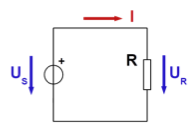
\includegraphics[height=2.5cm]{img/schaltung.png}
					\begin{itemize}\itemsep0pt				
						\item $R[\Omega]$
						\item $U_{R}=RI$
						\item $P=IU_{R}=\dfrac{U_{R}^{2}}{R}=RI^{2}$
					\end{itemize}
				\end{multicols*}
				\begin{itemize}\itemsep0pt
					\item Eine \textbf{Masche} oder Schlaufe ist irgendein Weg durch Drähte und Bauelemente, welche zu seinem Ausgangspunkt zurückführt.
					\item Die Spannung wird in Richtung Spannungsgefälle positiv gezählt, sonst negativ.
					\item Bei einem \textbf{Knoten} kommen mindestens drei Drähte zusammen.
					\item Durch die Ladungserhaltung muss die Summe der einfliessenden minus der Summe der wegfliessenden Ströme null ergeben.
					\item Kabelwiderstand $R = \rho\dfrac{L}{A}$							\end{itemize}			
				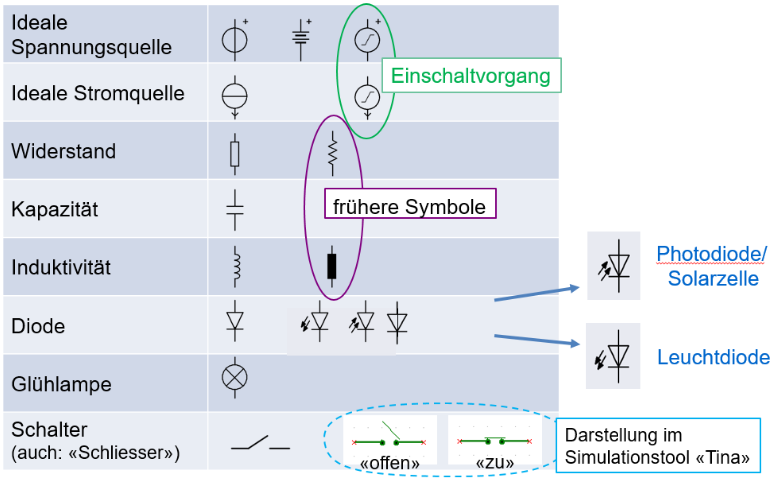
\includegraphics[height=4cm]{img/schaltung2.png}	
				\subsubsection{Serieschaltung}	
					\begin{itemize}\itemsep0pt
						\item Serieschaltung $R = R_{1} + R_{2}$
						\item Serieschaltung $I = \dfrac{U_{0}}{R_{1} + R_{2}}$
					\end{itemize}
				\subsubsection{Parallelschaltung}	
					\begin{itemize}\itemsep0pt
						\item Parallelschaltung $R=\dfrac{R_{1} \cdot R_{2}}{R_{1} + R_{2}}$
						\item Parallelschaltung $I_{0}=U_{0}(\dfrac{1}{R_{1}} + \dfrac{1}{R_{2}})$
					\end{itemize}
			
			
		\subsection{Batterie}
			\begin{multicols*}{2}
				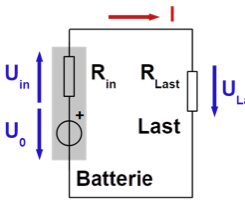
\includegraphics[height=2.5cm]{img/batterie.png} \\
				\begin{itemize}\itemsep0pt
					\item Ideale Bat: $U_{0}=const.$				
					\item $U_{0}-U_{in}-U_{last} =0$
					\item $U_{0}-IR_{in}-IR_{last} =0$
					\item $I=\dfrac{U_{0}}{R_{in}+R_{last}}$
					\item $P=R_{la.}(\dfrac{U_{0}}{R_{in}+R_{la.}})^{2}$
				\end{itemize}
			\end{multicols*}
			\begin{itemize}\itemsep0pt
				\item Wenn ein Verbraucher mit einer Batterie betrieben wird, muss aufgepasst werden, dass die Leistung nicht am Innenwiderstand der Batterie verbraucht wird.
				\item Bei einer Gleichspannungsquelle mit variabler Spannung, z.B. einer Solarzelle, muss der Lastwiderstand dynamisch anpasst werden (Bei Solarpaneln ist der Lastwiderstand der gleich wie beim Speicher).			
			\end{itemize}
			
		\subsection{Kondensator}
			\begin{multicols*}{2}
				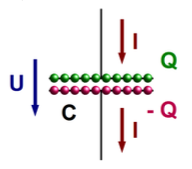
\includegraphics[height=2.9cm]{img/kondensator1.png} 
				
				\begin{itemize}\itemsep0pt
					\item Kondensatoren können praktisch beliebig oft aufge- und entladen werden.
					\item Kondensatoren können als Energiespeicher verwendet werden (Bremsenergie).
					\item Kapazität C [Farad/F]
					\item $\dfrac{\delta Q} {\delta t} = I$
					\item $CU_{c}=Q$
				\end{itemize}
				
			 \end{multicols*}
			 
			 \begin{multicols*}{2}
				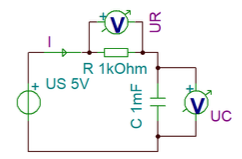
\includegraphics[height=2.2cm]{img/kondensator2.png} 
				
				\begin{itemize}\itemsep0pt
					\item $I = \dfrac{1}{R}(U_{s}-\dfrac{Q}{C})$
					\item $U_{s}=IR+\dfrac{Q}{C}$
				\end{itemize}
				
				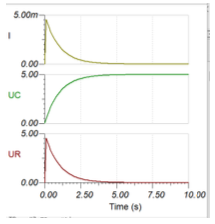
\includegraphics[height=3.5cm]{img/kondensator3.png} 

			 \end{multicols*}

		\subsection{Hochspannung}
			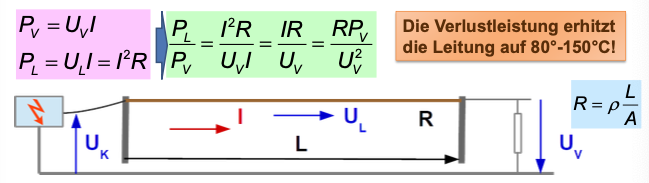
\includegraphics[height=2cm]{img/hochspannung1.png} 
			\begin{itemize}\itemsep0pt
				\item Je grösser $U_{V}, $desto kleiner der relative Leistungsverlust in der Leitung.
				\item Der Verlust beträgt wenige Prozent pro hunder Kilometer (Wechselspannung)
			\end{itemize}
			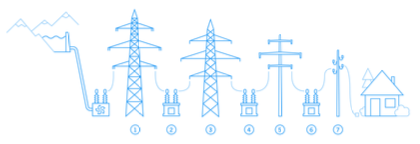
\includegraphics[height=2.2cm]{img/hochspannung2.png} 
			\begin{itemize}\itemsep0pt
				\item 1 Höchstspannung: 380 kV beziehungsweise 220 kV 
				\item 3 Hochspannungsebene: 36 kV bis 150 kV
				\item 5 Mittelspannungsebene: 1 kV bis 36 kV
				\item 7 Niederspannungsebene: $<$ 1 kV 
				\item 2,4,6 Transformatorenebenen 
			\end{itemize}
		\subsection{Gleich- und Wechselstrom}
			\begin{itemize}\itemsep0pt
				\item Historisch bedingt konnte früher nur Wechselstrom transformiert werden. 
				\item Wechselstrom relativ hohe Verlustleistung (Skineffekts, ..)
				\item Gleichstrom hat eine geringere Verlustleistung.
			\end{itemize}

		\section{Digitaltechnik}
			\subsection{Funktionseinheiten \& Signale}
				\begin{itemize}\itemsep0pt
					\item Eine \textbf{Funktionseinheit} empfangt n Inputsignale und liefert m Outputsignale
					\item Eine \textbf{Rückkopplung} ist beispielsweise wenn Outputsignal von FE1 Inputsignal von FE2 ist und ein Outputsignal von FE2 ein Inputsignal von FE1 ist.
					\item \textbf{Schaltnetze} enthalten mehrere Funktionseinheiten ohne Rückkopplungen.
					\item \textbf{Schaltwerk} enthalten Rückkopplungen und besitzen dadurch einen speichernden Charakter.
				\end{itemize}
			\subsection{Logik-Gatter}
				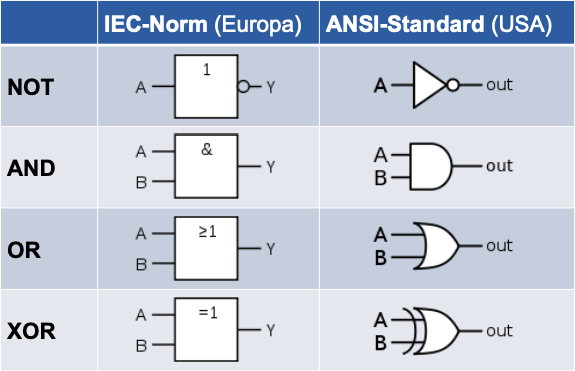
\includegraphics[height=4cm]{img/digitaleGrundbausteine.png} 
				\begin{itemize}\itemsep0pt
					\item Schalter die durch elektronische Signale betrieben werden sind \textbf{Transistoren}
					\item NOT: Einzelner Schalter
					\item AND: Zwei Schalter in serie
					\item OR: Zwei Schalter parallel
					\item XOR: Zwei Schalter in serie versetzt
				\end{itemize}
			
			\subsection{Flip-Flops}
			Ein Flip-Flop ist das fundamentale Speicherelement.
				\subsubsection{SR-Flip-Flop}
					\begin{itemize}\itemsep0pt
						\item Input S und R
						\item Funktioniert nur wenn S und R unterschiedlich oder beide Null sind (Beide Null speichert)
						\item Q = S
					\end{itemize}
					
				\subsubsection{D-Flip-Flop}
					\begin{itemize}\itemsep0pt
						\item S und R werden zu D zusammengefasst
						\item Wenn der Clockeingang von unten nach oben wechselt wird der Speicher gesetzt (flankengesteuert)
					\end{itemize}
					
				\subsubsection{JK-Flip-Flop}
					\begin{itemize}\itemsep0pt
						\item S wird mit J(Jump) und R mit K(Kill) ersetzt
						\item Es gibt einen Clockeingang (flankengesteuert)
						\item Wenn beide Eins sind, wechselt der Ausgang bei jeder aktiven Clockflanke
					\end{itemize}
					
			\subsection{KV-Diagramm}
				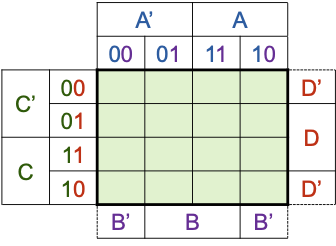
\includegraphics[height=5cm]{img/kv1.png} 
				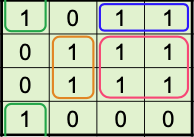
\includegraphics[height=2.5cm]{img/kv2.png} 
				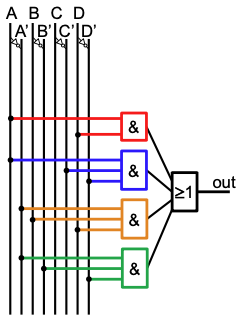
\includegraphics[height=4cm]{img/kv3.png} 


		\section{Elektrische und Magnetische Felder}

			\subsection{Ladungen und Ströme}
				\begin{itemize}\itemsep0pt
					\item Wenn man mehrere Ladungen hat, darf man die Kräfte zusammenzählen. Dies nennt man das Superpositionsprinzip.
					\item $\overrightarrow{F_{12}}$: Kraft auf Ladung $Q_{1}$, verursacht durch Ladung $Q_{2}$
					\item Einheitsvektor von $Q_{2}$ zu $Q_{1}$: $\overrightarrow{n}_{12} = \dfrac{\overrightarrow{r}_{12}}{|\overrightarrow{r}_{12}|}$
					\item Permittivität des Vakuums $ \varepsilon_{0}=8.859*10^{-12}\dfrac{C^{2}}{Jm}$
				\end{itemize}
			
			
			
			
			
			\subsection{Coulombgesetz}
				\begin{itemize}\itemsep0pt
					\item $\overrightarrow{F}_{12}=\dfrac{1}{4\pi\varepsilon_{0}}\dfrac{Q_{1}Q_{2}}{|\overrightarrow{r}_{12}|^{2}}\overrightarrow{n}_{12}$
				\end{itemize}
			
			\subsection{Elektrische Felder}
			
				\begin{itemize}\itemsep0pt
					\item $\overrightarrow{E}(\overrightarrow{r},t), [\dfrac{N}{C}]$
					\item Werden erzeugt durch Ladung oder zeitlich veränderliche magnetische Felder (Mehrer Quellen: Vektorsumme (Superpositionsprintzip))
				\end{itemize}
			
				Ladung $Q$ an Ort $\overrightarrow{r}_{Q}$ erzeug $\overrightarrow{E}$-Feld:		
				\begin{itemize}\itemsep0pt
					\item $\overrightarrow{E}(\overrightarrow{r}) = \dfrac{1}{4\pi\varepsilon_{0}} \dfrac{Q}{|\overrightarrow{r}-\overrightarrow{r}_{Q}|^{2}}  \dfrac{\overrightarrow{r}-\overrightarrow{r}_{Q}}{|\overrightarrow{r}-\overrightarrow{r}_{Q}|}$
					
				\end{itemize}
				Kraft auf Ladung q am Ort 
				$\overrightarrow{r}$:
				\begin{itemize}\itemsep0pt
					\item $\overrightarrow{F}=q\overrightarrow{E}(\overrightarrow{r},t)$
				\end{itemize}
			\subsection{Elektronvolt}
				\begin{itemize}\itemsep0pt
					\item $1 eV = W = F \cdot d =q\cdot E\cdot d=q \cdot U= 1.6\cdot10^{-19}J$
					\item Arbeit $W=\dfrac{m\cdot v^{2}}{2}$
				\end{itemize}
			\subsection{Magnetische Felder}
				\begin{itemize}\itemsep0pt
					\item $\overrightarrow{B}(\overrightarrow{r},t), [\dfrac{kg}{s\cdot C}]$
					\item Werden erzeugt durch Ströme oder zeitlich veränderliche elektrische Felder (Mehrer Quellen: Vektorsumme (Superpositionsprintzip))
					\item Das Magnetfeld zeigt vom Nord- zum Südpol
				\end{itemize}
				
				\subsubsection{Lorentzkraft}				
				
					\textbf{Lorentzkraft} auf Ladung q mit Geschwindigkeit $\overrightarrow{\nu}$:
					\begin{itemize}\itemsep0pt
						\item $\overrightarrow{F}_{L}=q\overrightarrow{\upsilon} $x$ \overrightarrow{B}$
					\end{itemize}	
					
					\textbf{Rechte Hand Regel}
					\begin{itemize}\itemsep0pt
						\item Mittelfinger: Richtung der Lorentzkraft
						\item Zeigefinger: Richtung des Magnetfeldes (Nord-Süd)
						\item Daumen: Richtung der positiven Ladung
					\end{itemize}					
				
			\subsection{Elektromotors}

\end{multicols*}

% Dokumentende
% ======================================================================
\end{document}
